\icode{E-MI-MU-L3-261113-002}
（多选）
在竖直固定的光滑绝缘圆环轨道上，套着两带电小环 $a$、$b$。两小环处于静止状态，且刚好位于同一水平线上。若小环 $b$ 缓慢漏电，则\paren[]

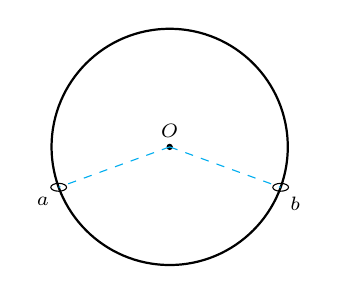
\begin{tikzpicture}[font=\scriptsize]
	\draw[thick] (0,0) circle(1.5);
	\fill (0,0)node[above]{\(O\)} circle(0.04);
	\draw[dashed,cyan] (0,0)--++(-160:1.5)coordinate(a) (0,0)--++(-20:1.5)coordinate(b);
	\draw (a)node[below left]{\(a\)} ellipse(.1 and .05) (b)node[below right]{\(b\)} ellipse(.1 and .05);
\end{tikzpicture}
\begin{choices}
	\item 漏电前，$a$、$b$ 两小环质量和电量均相同
	\item 漏电过程中，小环 $a$ 对轨道的压力大小不变
	\item 漏电过程中，两小环始终在同一高度且库仑力逐渐减小
	\item 漏电过程中，若小环 $a$ 固定，则小环 $b$ 受到轨道的支持力逐渐增大
\end{choices}
\begin{answer}
	AC\qquad 提示：
\end{answer}